\chapter{Testy i porównanie algorytmów}
\section{Analiza działania poszczególnych algorytmów}
\subsection{Algorytm Roju Cząsteczek}
\subsubsection{Problemy związane z rozwiązaniem}
\par Podczas analizy oraz testowania zaimplementowanego rozwiązania, okazało się, że algorytm jest mało skuteczny, gdyż nie był w stanie usunąć całkowicie naruszeń ograniczeń twardych. Ograniczenia te w bezpośredni sposób wpływają na prawidłowość wygenerowanego planu zajęć.
\par W związku z tym zdecydowałem się na wprowadzenie dodatkowej kary: do kary za ograniczenia miękkie dodaję za każde naruszenie ograniczenia twardego 1 milion punktów kary. Dzięki temu, algorytm w pierwszej kolejności bierze pod uwagę ograniczenia twarde, próbując je wyeliminować, a potem dopiero ograniczenia miękkie. \\

Poniższy wykres pokazuje efektywność algorytmu. Uwagę należy zwrócić na skalę przyjętą na osi y. Wartości nie schodzą poniżej $10^{7}$ czyli wynik w najlepszym wypadku nadal łamie 10 twardych ograniczeń.

\begin{figure}[H]
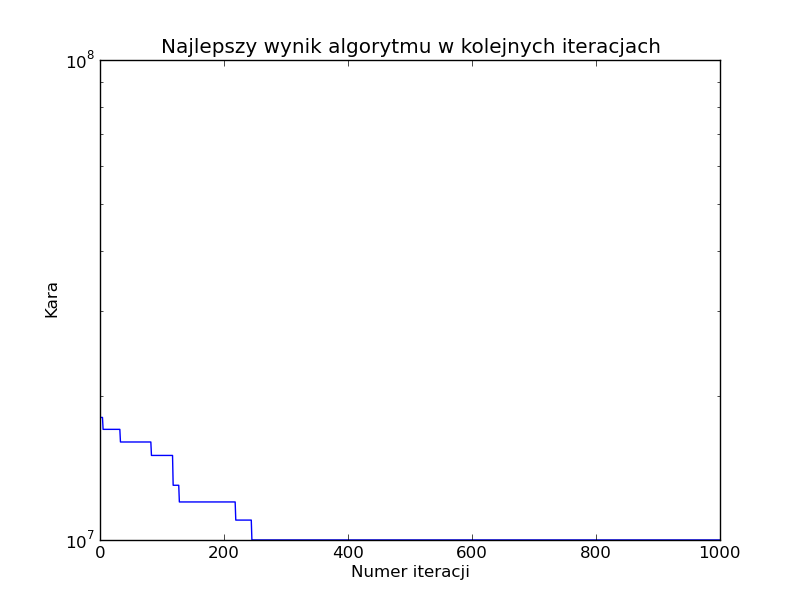
\includegraphics[width=10cm]{img/standard_penalty.png}
\centering
\end{figure}
\par W celu sprawdzenia przyczyny tego zachowania przyjrzałem się zachowaniu pojedynczej cząsteczki. Okazało się, że kara za kolejno generowane plany oscyluje wokół kary wyliczonej dla początkowego planu, co potwierdza poniższy wykres.  
\begin{figure}[H]
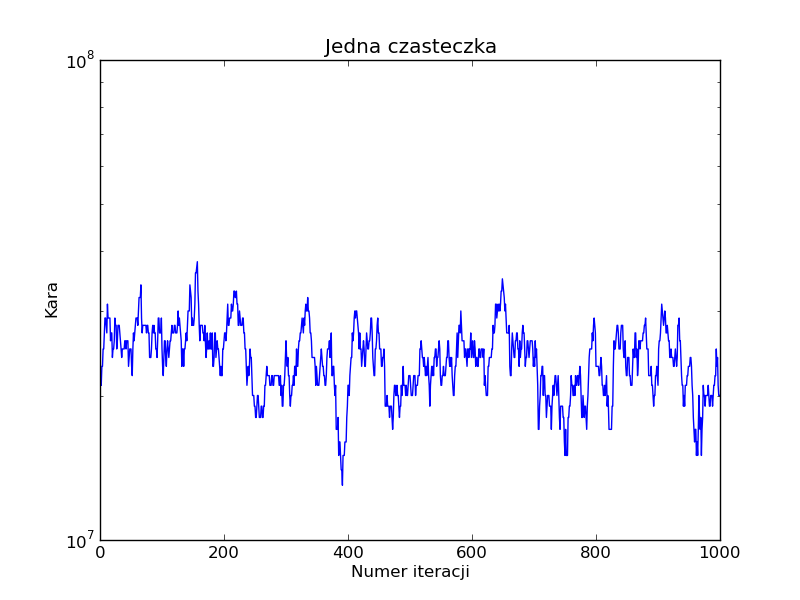
\includegraphics[width=10cm]{img/standard_particle.png}
\centering
\end{figure}
\par Na podstawie dalszej analizy okazało się, że wszystkie cząsteczki zachowują się bardzo podobnie, co można zaobserwować na wykresie. 
\begin{figure}[H]
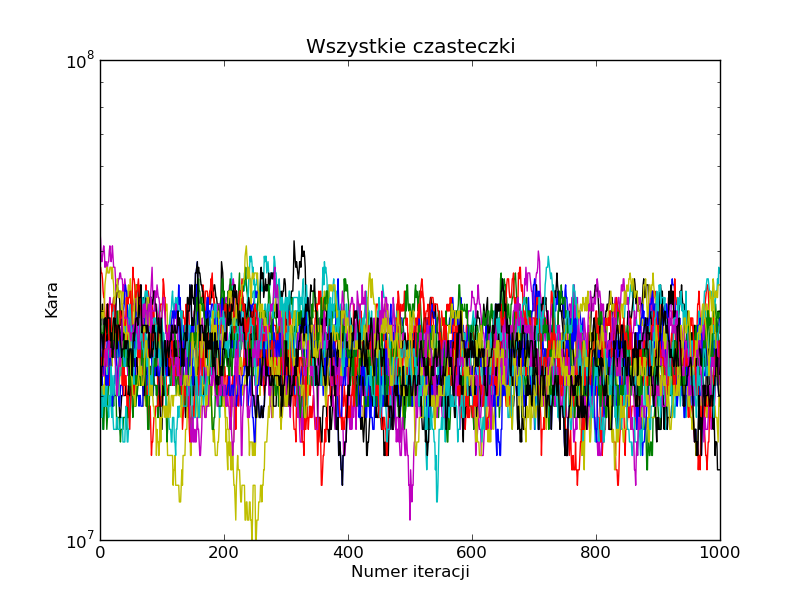
\includegraphics[width=10cm]{img/standard_particle_all.png}
\centering
\end{figure}
\subsubsection{Modyfikacje}
\par W celu dojścia do lepszego rozwiązania problemu układania planu zajęć za pomocą algorytmu PSO, rozważyłem dwie modyfikacje zaproponowanego wcześniej algorytmu.Pierwsza z nich to  ,,podążanie za lokalnie najlepszym planem'', a druga zaś ,,podążanie za globalnie najlepszym planem''. Obie modyfikacje są analogiczne do siebie, jedyną ich różnicą jest tylko plan, który jest brany pod uwagę. Dokonałem również modyfikacji fazy dotyczącej oceny aktualnego rozwiązania, która jest przeprowadzana na początku każdej iteracji. Ponadto został dodany warunek, że jeśli aktualny plan jest gorszy od najlepszego planu to zostaje on zamieniony na najlepszy plan. Zrezygnowałem również z realizacji krotów 3 i 4, opisanych w algorytmie PSO.

\par W przypadku gdy każda cząsteczka ,,podąża za swoim lokalnie najlepszym planem'' istnieje mniejsze ryzyko, że algorytm pozostanie w lokalnym minimum przestrzeni rozwiązań. Natomiast podczas ,,podążania za globalnie najlepszym planem'' algorytm będzie znacznie szybciej dążył do najbliższego minimum.

\par Opcja ,,podążania za lokalnie najlepszym planem'' okazała się być dużo efektywniejsza od podstawowego algorytmu. W tym przypadku twarde ograniczenia nie były naruszone, co potwierdza poniższy wykres.
\begin{figure}[H]
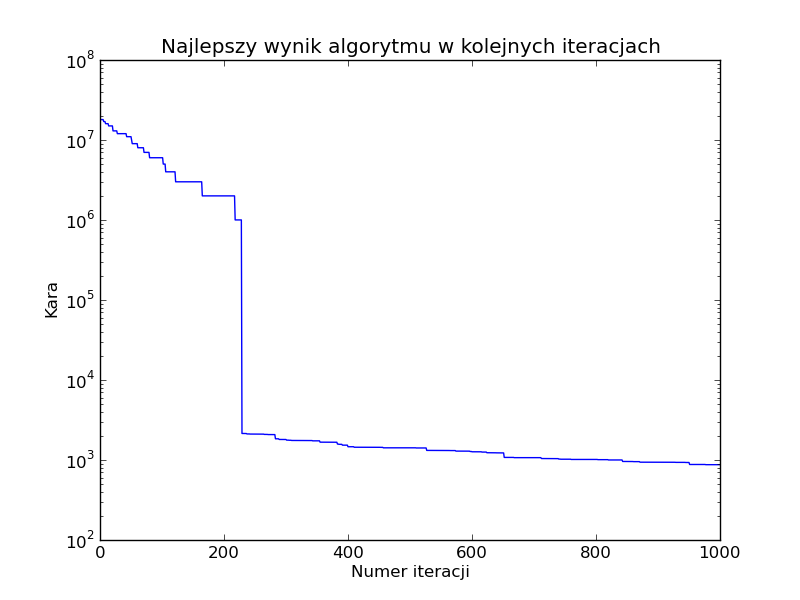
\includegraphics[width=10cm]{img/localbest_penalty.png}
\centering
\end{figure}
\par Analizując pojedynczą cząsteczkę można zauważyć, że kara często zmienia się od małych wartości do wartości powyżej miliona. Spowodowane jest to tym, że po zamianie dwóch lekcji w poprzedniej iteracji pojawił się konflikt z twardymi ograniczeniami. W tej sytuacji algorytm powraca do poprzedniego rozwiązania. Na poniższych wykresach widać zachowanie dla pojedynczej cząsteczki oraz dla wszystkich cząsteczek.
\begin{figure}[H]
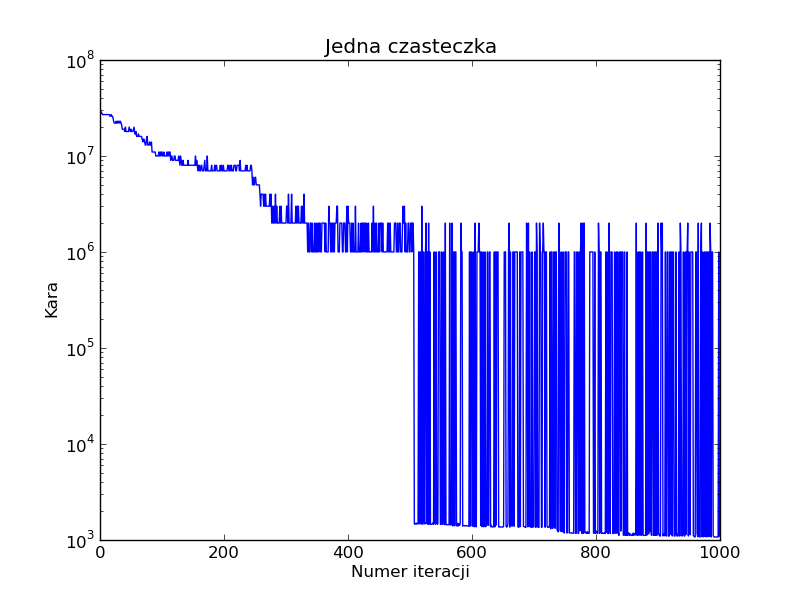
\includegraphics[width=10cm]{img/localbest_particle.png}
\centering
\end{figure}
\begin{figure}[H]
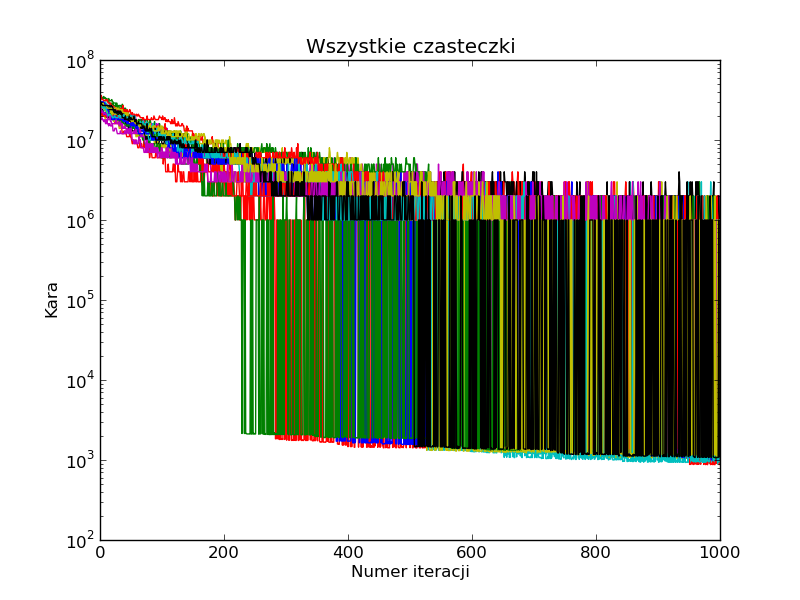
\includegraphics[width=10cm]{img/localbest_particle_all.png}
\centering
\end{figure}
\par Opcja podążania za globalnie najlepszym planem okazała się być bardziej efektywna. Sporym zaskoczeniem był brak problemów z lokalnymi minimami przestrzeni rozwiązań. Poniższy wykres pokazuje skuteczność modyfikacji.
\begin{figure}[H]
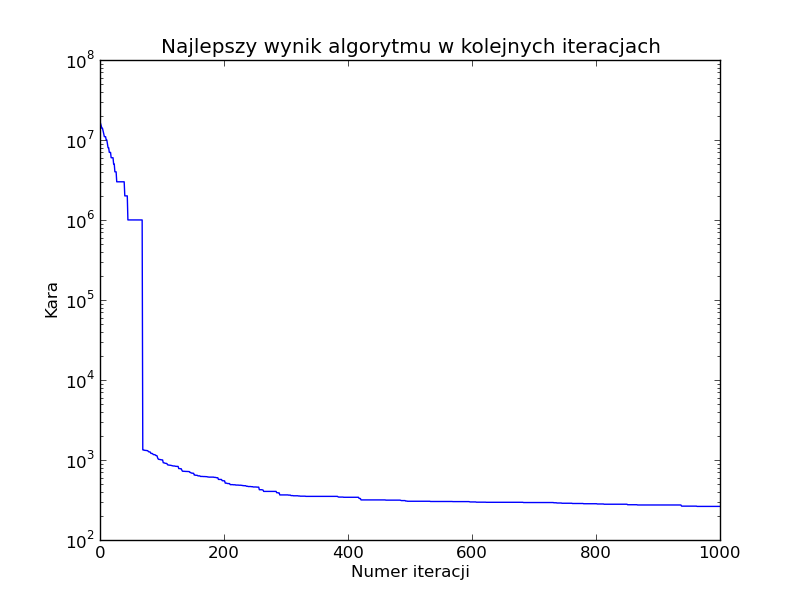
\includegraphics[width=10cm]{img/globalbest_penalty.png}
\centering
\end{figure}
\par W tym przypadku cząsteczki zachowywały się bardzo podobnie. Jedyną różnicą była prędkość z jaką malała funkcja kary, można to zauważyć na poniższych wykresach. 

\begin{figure}[H]
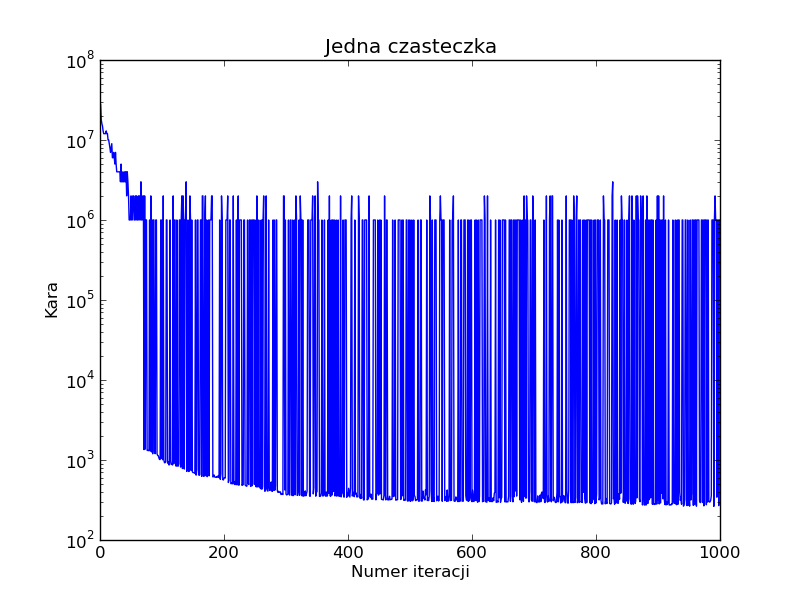
\includegraphics[width=10cm]{img/globalbest_particle.png}
\centering
\end{figure}

\begin{figure}[H]
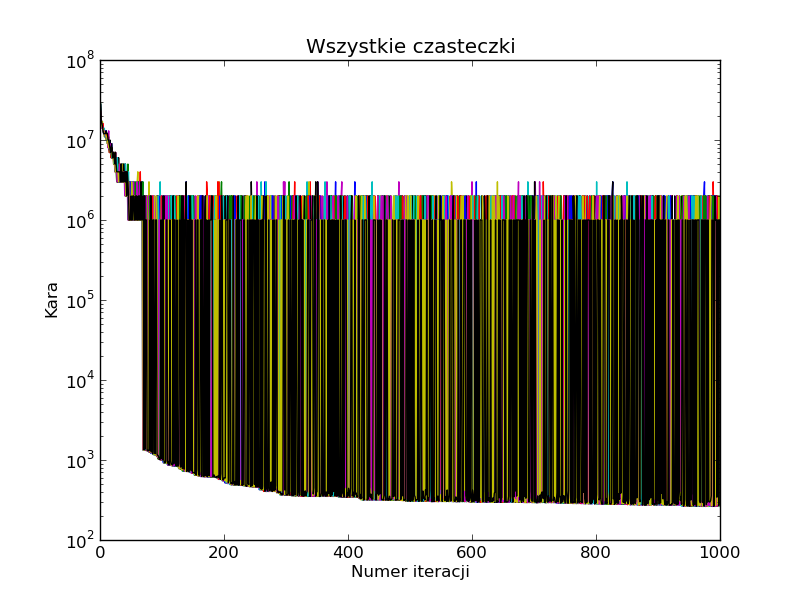
\includegraphics[width=10cm]{img/globalbest_particle_all.png}
\centering
\end{figure}

\subsubsection{Ostateczne rozwiązanie}

\par Jako ostateczne rozwiązanie wybrałem podążanie za globalnie najlepszym planem. Jest to spowodowane tym, że mimo wielu testów nie udało mi się znaleźć przypadku kiedy podążanie za lokalnie najlepszym planem wypadłoby lepiej. 
\subsection{Algorytm Adaptacyjny Tabu}
Przedstawienie działania algorytmu dla wybranych testów.\\
Testy szczegółowo zostały opisane w kolejnej sekcji.
\par \textbf{Test 1}
\begin{figure}[H]
  \caption{Wykres zależności funkcji oceny od czasu}
  \centering
    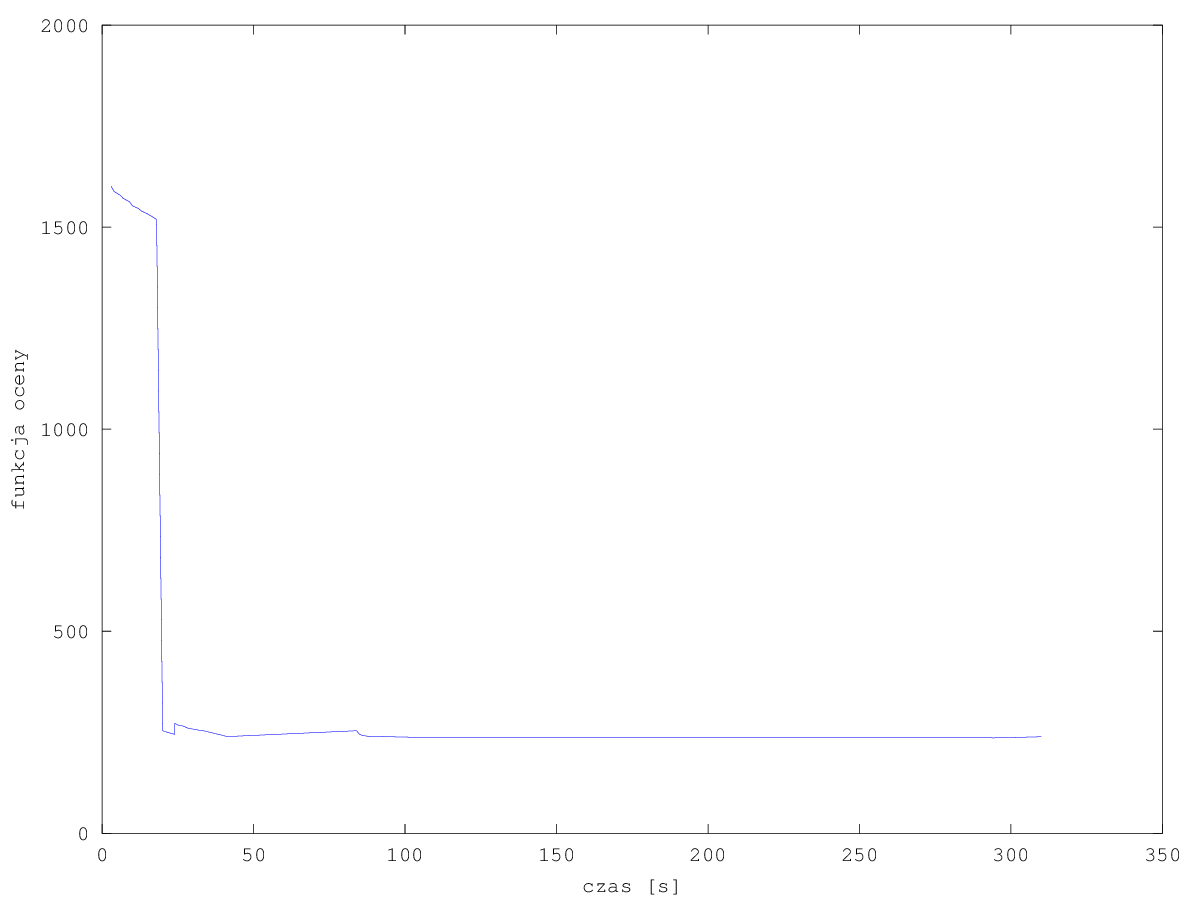
\includegraphics[width=10cm]{ogolny.png}
\end{figure}
Na wykresie wyraźnie widać wyodrębioną fazę inicjalizacji, w której tworzone jest początkowe rozwiązanie nienaruszające twardych ograniczeń. Nagła zmiana wartości funkcji oceny wynika z wywołania w algorytmie funkcji przypasowującej sale do poszczególnych zajęć. Celem tej funkcji jest początkowe przypasowanie największych sal do kursów, na które uczęszcza największa liczba studentów, dzięki temu zmiejszana jest funkcja oceny miękkich ograniczeń dotycząca wielkości sali wykładowej. Stosunkowo długi czas działania algorytmu wynika z bardzo dużej ilości wywołań funkcji oceny, niezbędnej do stworzenia rozwiązania początkowego oraz do określenia najlepszych mozliwych zmian, które mogą zostać wprowadzone w kolejnych fazach: intensyfikacji i dywersyfikacji. Problem mógłby zostać rozwiązany implementacją modułu w języku \verb#C#, który w znacznie szybszy sposób wylicza funkcję kary, niż zaimplementowana optymalnie ta sama funkcjonalność w języki \verb#python#.
\begin{figure}[H]
  \caption{Wykres zależności funkcji oceny od czasu, bez uwzględnienia fazy inicjalizacji}
  \centering
    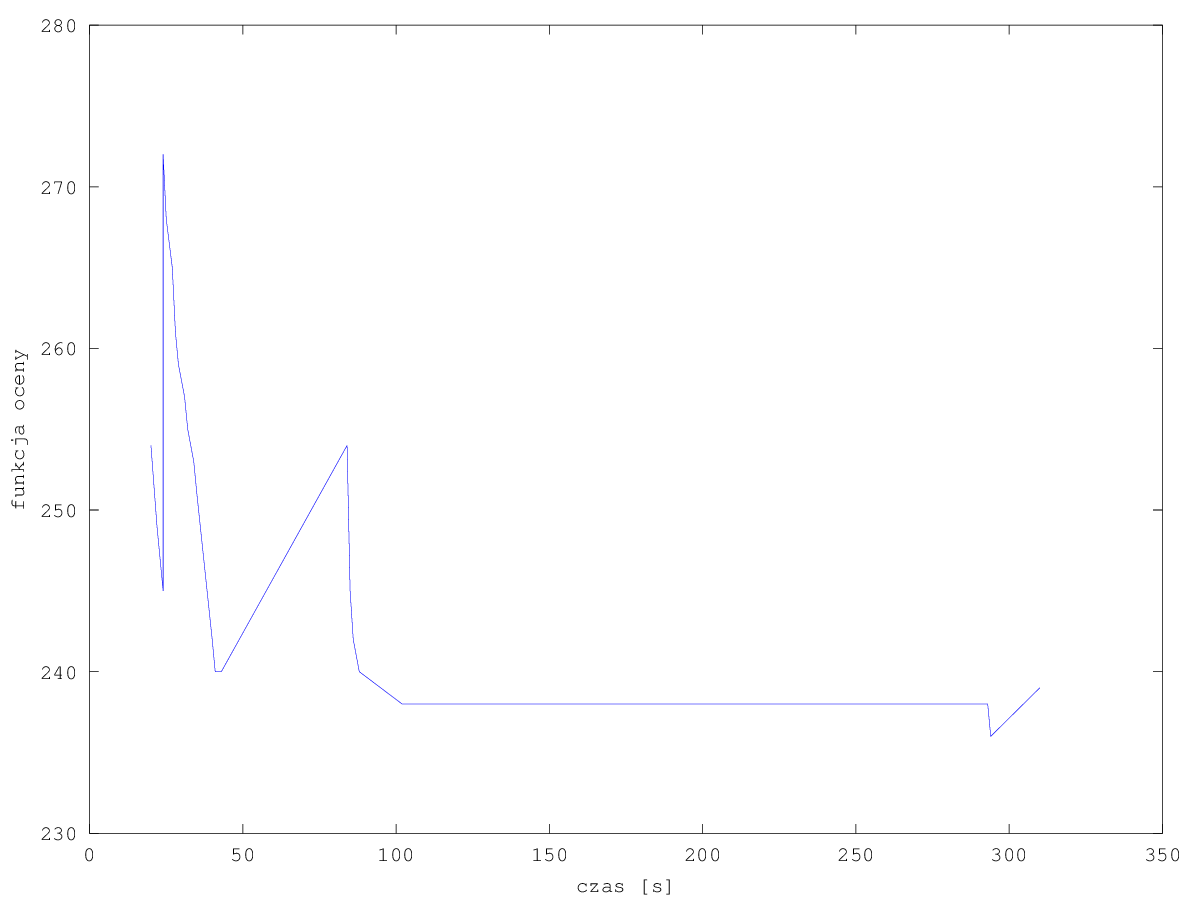
\includegraphics[width=10cm]{szczeg.png}
\end{figure}
Wykres ten obrazuje działanie losowego operatora zaburzeń w fazie dywersyfikacji, którego celem jest zniszczenie osiągniętego lokalnego minimum.
\par \textbf{Test 2}
\begin{figure}[H]
  \caption{Wykres zależności funkcji oceny od czasu}
  \centering
    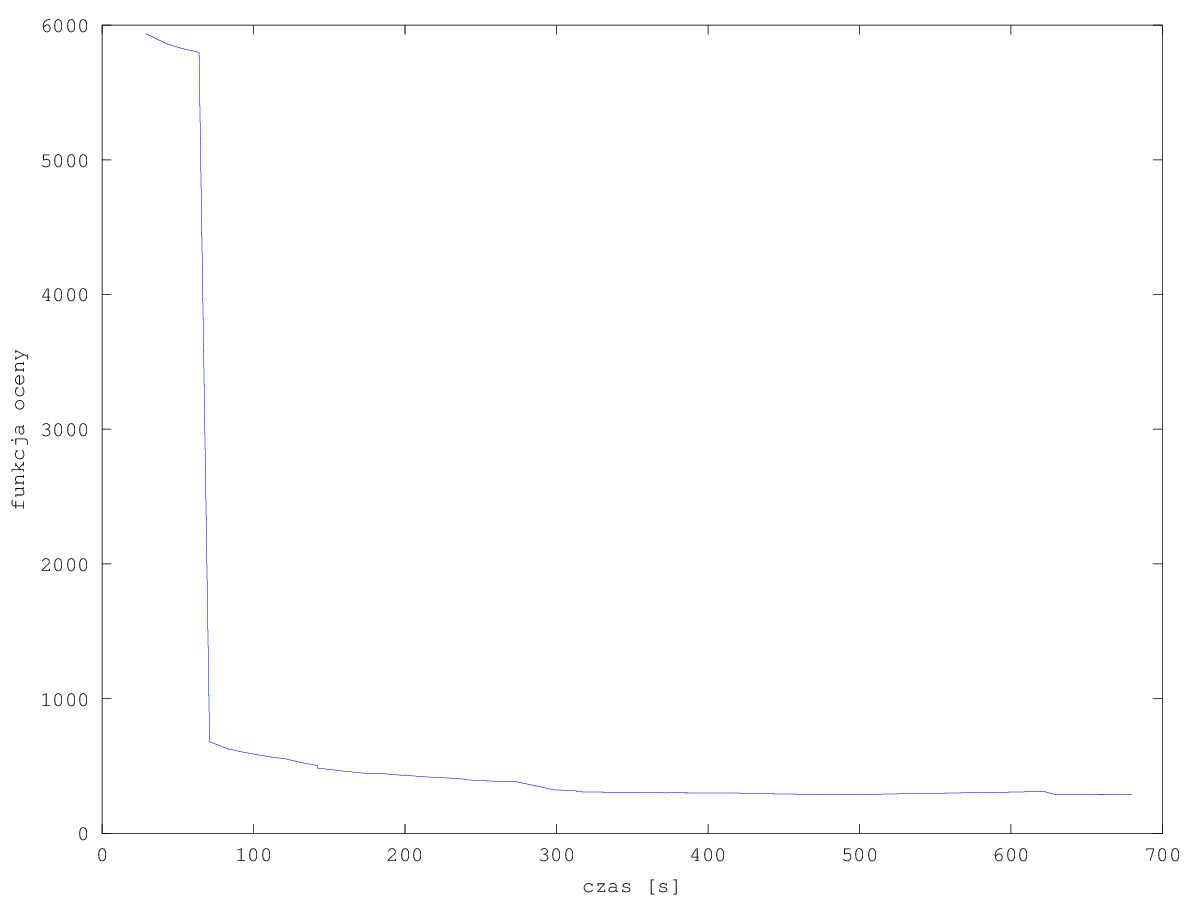
\includegraphics[width=10cm]{ogolny2_instancja.png}
\end{figure}
Wykres obrazuje jak zmieniała się funkcja oceny w czasie. Dla testu 2 początkowe rozwiązanie zostało stworzone w czasie 29 sekund zaś dla testu 1 w czasie 3 sekund. Czas tworzenia początkowego rozwiązania jest ściśle związany ze złożonością danych wejściowych: liczbą kursów, programów nauczania, dostępnych sal i dodatkowych ograniczeń. Drugi test jest znacznie bardziej złożony niż test 1, dlatego też czas wykonania fazy inicjalizacji jest znacznie dłuższy.
\begin{figure}[H]
  \caption{Wykres zależności funkcji oceny od czasu, bez uwzględnienia fazy inicjalizacji}
  \centering
    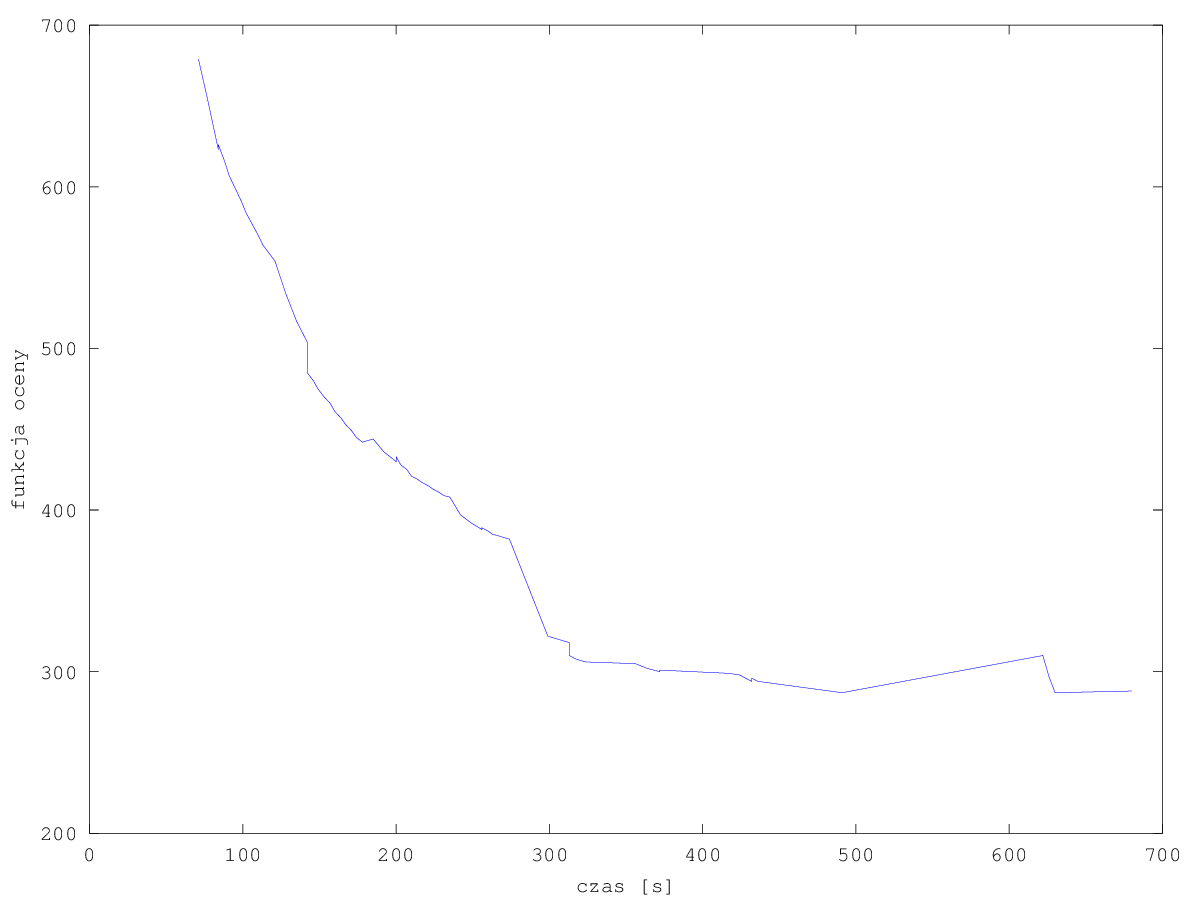
\includegraphics[width=10cm]{szczegolowy2_instancja.png}
\end{figure}
Wykres przedstawiający działanie algorytmu w fazie dywersyfikacji i intensyfikacji.
\section{Specyfikacja testów}
\textit{Katarzyna Śmietanka} 
\\
Dane testowe pobrane zostały z konkursu ,,International Timetabling Competition 2007''. Do oceny rozwiązań używany jest oryginalny walidator rozwiązań, zapewniony przez organizatorów konkursu.
\par Poworównanie działania poszczególnych algorytmów okazało się być stosunkowo trudne, ze względu na różnorodność zaimplementowanych przez nas algorytmów. Algorytm Adaptacyjny Tabu ma odmienne iteracje niż Algorytm Genetyczny czy też Roju Cząsteczek. Ponadto wpływowym czynnikiem na szybkość działania algorytmu jest sposób implementacji, a jest on odmienny dla każdego z naszych algorytmów. Dodatkowo część z nas korzystała z wbudowanych funkcji z języka \verb#python# oraz programowania funkcjonalnego, które w znaczny sposób przyspieszają wykonywanie złożonych operacji. Dlatego też zdecydowaliśmy się, że każdy z algorytmów dla poszczególnych instancji zostanie uruchomiony z najlepszymi, zaobserwowanymi parametrami, dla których uzyskane rozwiązanie jest optymalne. Dla poszczególnych instancji zostanie przedstawiona szczegółowa specyfikacja danych testowych, wyniki działania algorytmów oraz wykresy zależności funkcji oceny od liczby odwołań do tej funkcji oceny.
\subsection{Test 1}
\begin{table}[H]
\begin{center}
 
\begin{tabular}{ |l|l| }
\hline
$Liczba\ kursów$ & $30$\\
\hline
$Liczba\ programów\ nauczania$ & $14$\\
\hline
$Liczba\ dni$ & $5$ \\
\hline
$Licza\ przedziałów\ czasowych$ & $6$ \\
\hline
$Liczba\ ograniczeń$ & $53$ \\
\hline
$Liczba\ sal$ & $6$ \\
\hline
\end{tabular}
\end{center}
\end{table}

\par Wyniki działania algorytmów- ocena wygenerowanych planów zajęć: \\
Parametry dla algorytmów:
\begin{enumerate}
\item GA - liczba osobników: 100, liczba iteracji: 500, szacowany czas działania algorytmu: 150 s
\item PSO - liczba cząsteczek: 20, liczba iteracji 10000, szacowany czas działania algorytmu: 40 min
\item ATS - czas działania: 120 s
\end{enumerate}
\begin{table}[H]
\begin{center}

\begin{tabular}{ |l|l|l|l| }
\hline
 & $GA$ & $PSO$ & $ATS$\\
\hline
${H}_{1}\ Wykłady$ & $0$ & $0$ & $0$\\
\hline
$H_{2}\ Zajętość\ sali$ & $0$ & $0$ & $0$\\
\hline
$H_{3}\ Konflikty\ pomiędzy\ kursami$ & $0$ & $0$ & $0$ \\
\hline
$H_{4}\ Dostępność\ wykładowcy$ & $0$ & $0$ & $0$ \\
\hline
$S_{1}\ Wielkość\ sali$ & $4$ & $5$ & $205$ \\
\hline
$S_{2}\ Stabilność\ pomieszczenia$ & $14$ & $24$ & $32$ \\
\hline
$S_{3}\ Minimalna\ liczba\ dni$ & $0$ & $0$ & $0$ \\
\hline
$S_{4}\ Zwartość\ zajęć$ & $56$ & $8$ & $6$ \\
\hline
$Funkcja\ oceny$ & $74$ & $37$ & $243$ \\
\hline
\end{tabular}
\end{center}
\caption {Wyniki uzyskane przez poszczególne algorytm}
\end{table}
\par Jak można zaobserwować najlepszy rezultat dla pierwszej instancji uzyskał algorytm PSO, jednak czas potrzebny do uzyskania tego wyniku był stosunkowo długi w porównaniu do algorytmu GA. Żaden z wygenerowanych planów nie narusza ograniczeń twardych. Najgorsze wyniki uzyskał Algorytm Adaptacyjny Tabu, prawdopodobnie czas działania algorymu był zbyt krótki, tak aby zmiejszyć funkcję oceny.
\par Ciekawym spostrzeżeniem jest to, że żaden z algorytmów nie miał problemu z minimalizacją do zera ograniczenia miękkiego,  $S_{3}$, które dotyczy minimalnej liczby dni na które muszą być rozłożone zajęcia z danego kursu. Kara uzyskana za $S_{2}$ stabilnośc pomieszczenia jest porównywalna dla wszystkich algorytmów.
\par  Wykresy zmiany funkcji oceny w zależności od liczby odwołań do funkcji oceny dla poszczególnych algorytmów. 
\begin{figure}[H]
  \caption{Algorytm Genetyczny}
  \centering
    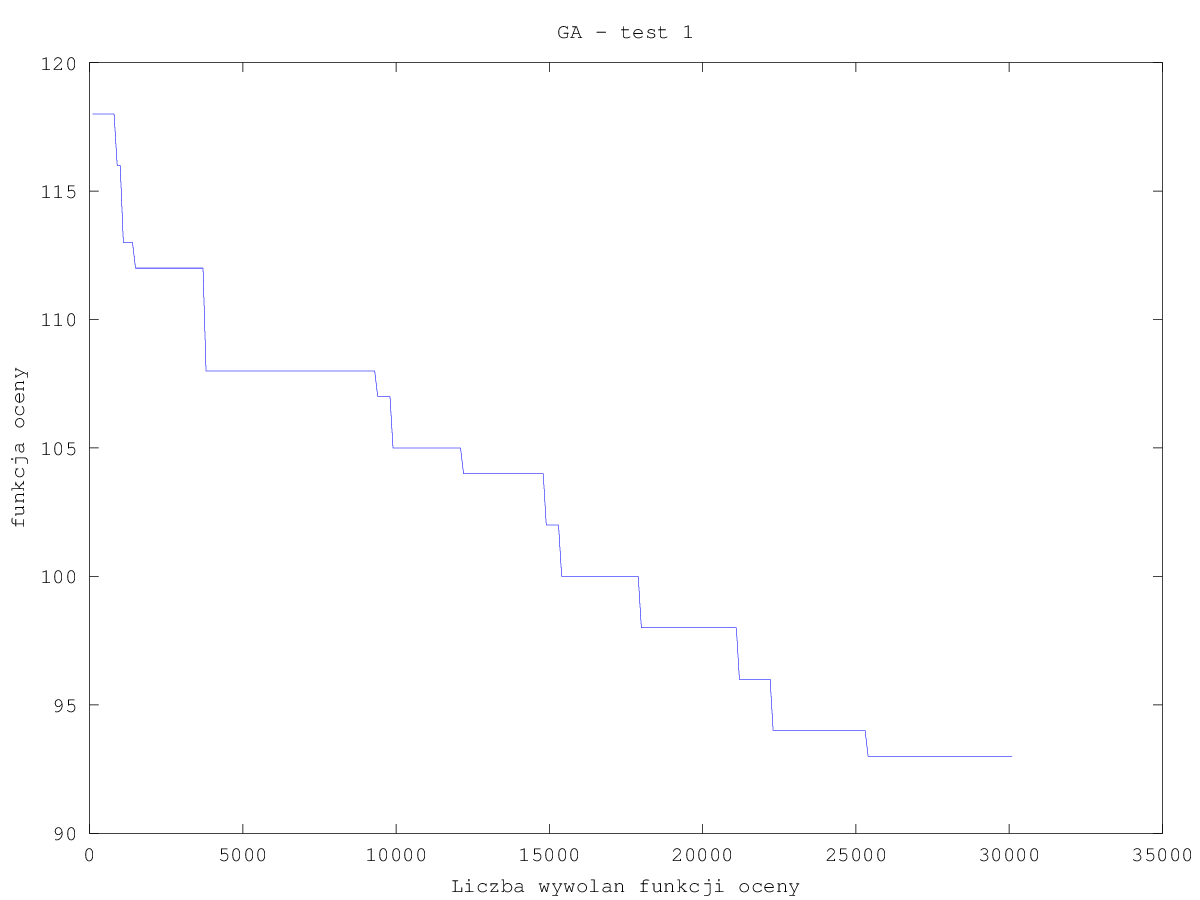
\includegraphics[width=10cm]{ga_test_1.png}
\end{figure}
\begin{figure}[H]
  \caption{Algorytm Roju Cząsteczek}
  \centering
    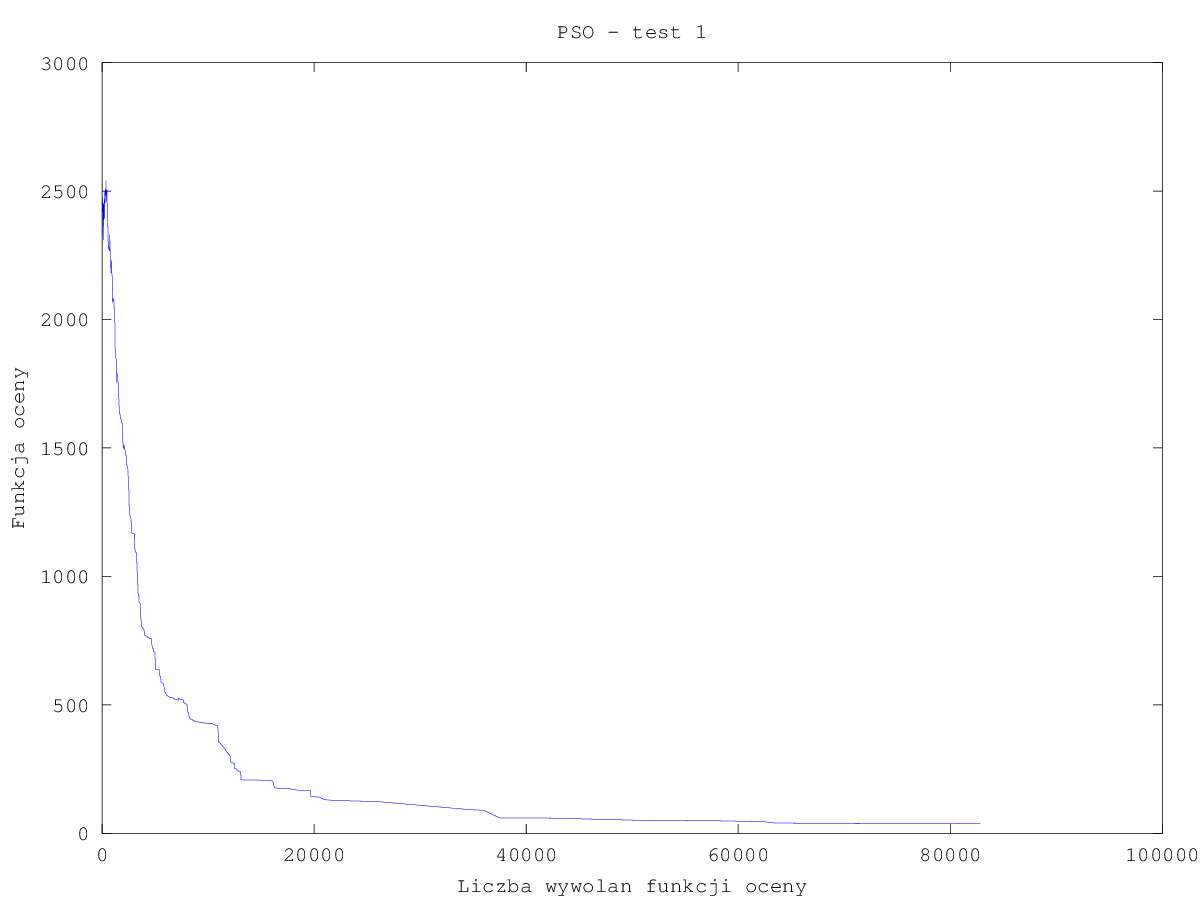
\includegraphics[width=10cm]{pso_1.png}
\end{figure}
\begin{figure}[H]
  \caption{Algorytm Adaptacyjny Tabu}
  \centering
    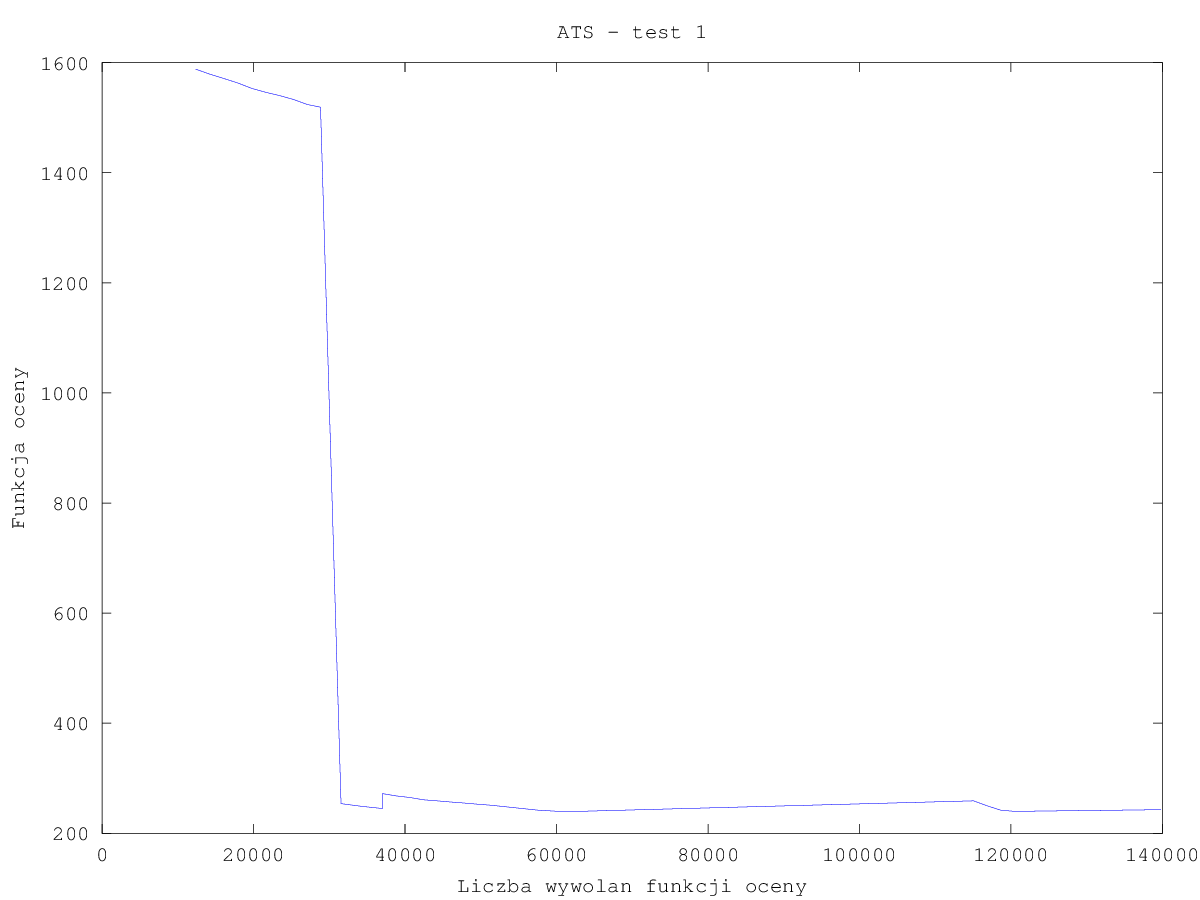
\includegraphics[width=10cm]{ats_test_1.png}
\end{figure}
W powyższych wykresów można zaobserwować funkcję oceny początkowych rozwiązań wygenerowanych przez każdy z algorytmów. Najniższą wartość oceny na początku uzyskał algorytm GA, najwyższą zaś PSO. Dla każdego z wywołań alorytmu GA, czy też PSO funkcja oceny rozwiązania początkowego będzie inna, ze względu na losowość zaś w algorytmie ATS taka sama. W ATS początkowe rozwiązanie jest tworzone przy pomocy heurystyki, która w ten sam sposób, dla tej samej instancji tworzy inicjalny plan zajęć. Ciekawą cechą algorytmu ATS jest stosunkowo duża liczba odwołań algorytmu do funkcji oceny, choćby dla początkowej fazy działania algorytmu. Wykres funkcji oceny od liczby referencji dla PSO ma kształt wykresu funkcji wykładniczej malejącej. Nietypowy kształ wykresu dla ATS wynika z nagłej zmiany najlepszego rozwiązania, spowodowanej wywołaniem funkcji przypasowującej sale do poszczególnych zajęć. 
\subsubsection{Test 1 - wizualizacja}
Celem stworzenia wizualizacji jest zobrazowanie instancji problemu, jak również pokazanie, że wprowadzanie kolejnych nawet minimalnych ograniczeń znacznie komplikuje problem.
\begin{figure}[H]
  \caption{Graf przedstawiający wszystkie zależności pomiędzy kursami (uwzględniając tych samych prowadzących nauczycieli oraz należenie kursu do tego samego programu nauczania) }
  \centering
    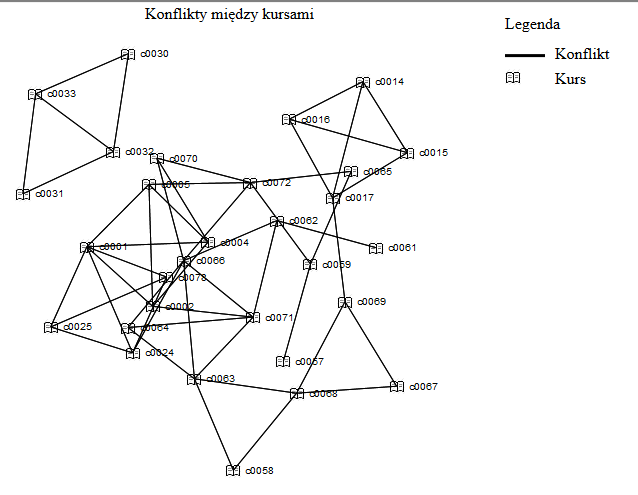
\includegraphics[width=10cm]{test1.PNG}
\end{figure}
\par Oddzielne przestawienie poszczególnych ograniczeń na grafach\\ Wierzchołkami są kursy, a krawędzie są to konflikty pomiędzy kursami, oznaczające, że zajęcia z kursów połączonych krawędzią nie mogą odbywać się w tym samym czasie.

\begin{figure}[H]
  \caption{Graf uwzględniający zależności pomiędzy kursami uwzględniając prowadzących dane kursy}
  \centering
    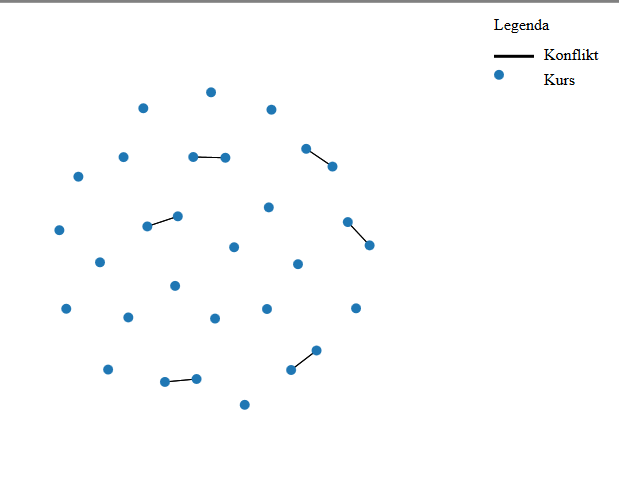
\includegraphics[width=10cm]{test1_teach.PNG}
\end{figure}
\begin{figure}[H]
  \caption{Graf uwględniający grupy zależnych od siebie kursów wchodzących w skład tego samego programu nauczania}
  \centering
    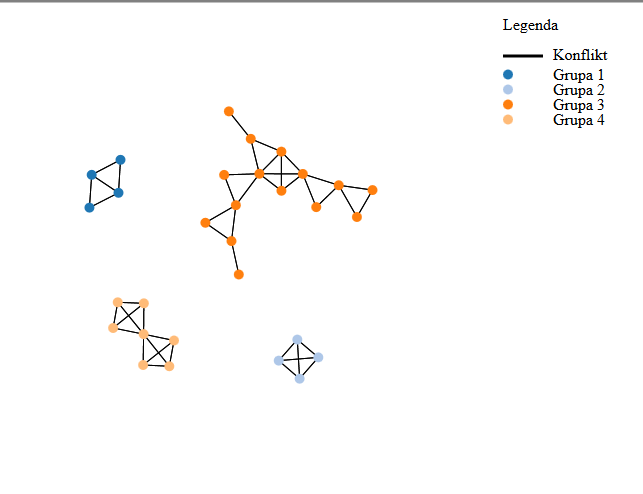
\includegraphics[width=10cm]{test1_con.PNG}
\end{figure}
\subsection{Test 2}
\begin{table}[H]
\begin{center}

\begin{tabular}{ |c|c|c|c| }
\multicolumn{1}{r}{}
 &  \multicolumn{1}{c}{$$}
 & \multicolumn{1}{c}{$$} 
 \\
\cline{1-2}
$Liczba\ kursów$ & $82$\\
\cline{1-2}
$Liczba\ programów\ nauczania$ & $70$\\
\cline{1-2}
$Liczba\ dni$ & $5$ \\
\cline{1-2}
$Licza\ przedziałów\ czasowych$ & $5$ \\
\cline{1-2}
$Liczba\ ograniczeń$ & $513$ \\
\cline{1-2}
$Liczba\ sal$ & $16$ \\
\cline{1-2}
\end{tabular}
\end{center}
\caption {Specyfikacja danych - Test 2}
\end{table}
\par Wyniki działania algorytmów- ocena wygenerowanych planów zajęć: \\
Parametry dla algorytmów:
\begin{enumerate}
\item GA - liczba osobników: 200, liczba iteracji: 1000, szacowany czas działania algorytmu: 33 min
\item PSO - liczba cząsteczek: 20, liczba iteracji 10000, szacowany czas działania algorytmu: 180 min
\item ATS - czas działania: 10 min
\end{enumerate}
\begin{table}[H]
\begin{center}

\begin{tabular}{ |l|l|l|l| }
\hline
 & $GA$ & $PSO$ & $ATS$\\
\hline
${H}_{1}\ Wykłady$ & $0$ & $1$ & $0$\\
\hline
$H_{2}\ Zajętość\ sali$ & $0$ & $0$ & $0$\\
\hline
$H_{3}\ Konflikty\ pomiędzy\ kursami$ & $0$ & $0$ & $0$ \\
\hline
$H_{4}\ Dostępność\ wykładowcy$ & $0$ & $2$ & $0$ \\
\hline
$S_{1}\ Wielkość\ sali$ & $119$ & $54$ & $0$ \\
\hline
$S_{2}\ Stabilność\ pomieszczenia$ & $63$ & $51$ & $143$ \\
\hline
$S_{3}\ Minimalna\ liczba\ dni$ & $70$ & $74$ & $40$ \\
\hline
$S_{4}\ Zwartość\ zajęć$ & $424$ & $150$ & $104$ \\
\hline
$Funkcja\ oceny$ & $676$ & $330$ & $287$ \\
\hline
\end{tabular}
\end{center}
\caption {Wyniki uzyskane przez poszczególne algorytmy}
\end{table}
Jak można zauważyć z powyższej tabeli algorytm PSO mimo bardzo długiego czasu działania nie usunął wszystkich naruszeń związanych z ograniczeniami twardymi dotyczącymi: ${H}_{1}$ przyporządkowania wszystkich wykładów oraz $H_{4}$ dostępności wykładowcy. Najlepszy rezultat działania został uzyskany przez ATS, którego czas działania był najkrótszy w stosunku do pozostałych algorytmów. Największym problemem do minimalizacyjnym dla wszystkich algorytmów było zmiejszenie funkcji oceny za $S_{4}$ zwartość zajęc, a kara otrzymana za $S_{3}$ jest porównywalna dla wszystkich algorytmów. 
Zarówno Algorytm Genetyczny jak również Algorytm Róju cząsteczek nie dają gwarancji wygenerowania całkowicie poprawnego planu zajęć, nie naruszającego żadnych z ograniczeń $H_{1}-H_{4}$. Algorytm Adaptacyjny Tabu gwarantuje, że ograniczenia $H_{2}-H_{4}$ będą spełnione dla stworzonego planu zajęć, ale nie zapewnia o spełnieniu ograniczenia ${H}_{1}$. Nie spełnienie tego ograniczenia może zajść w fazie inicjalizacji, gdzie nie będzie możliwe przyporządkowanie zajęć do żadnego z przedziałów czasowych nie naruszając innych ograniczeń.
\par  Wykresy zmiany funkcji oceny w zależności od liczby odwołań do funkcji oceny dla poszczególnych algorytmów.
\begin{figure}[H]
  \caption{Algorytm Genetyczny}
  \centering
    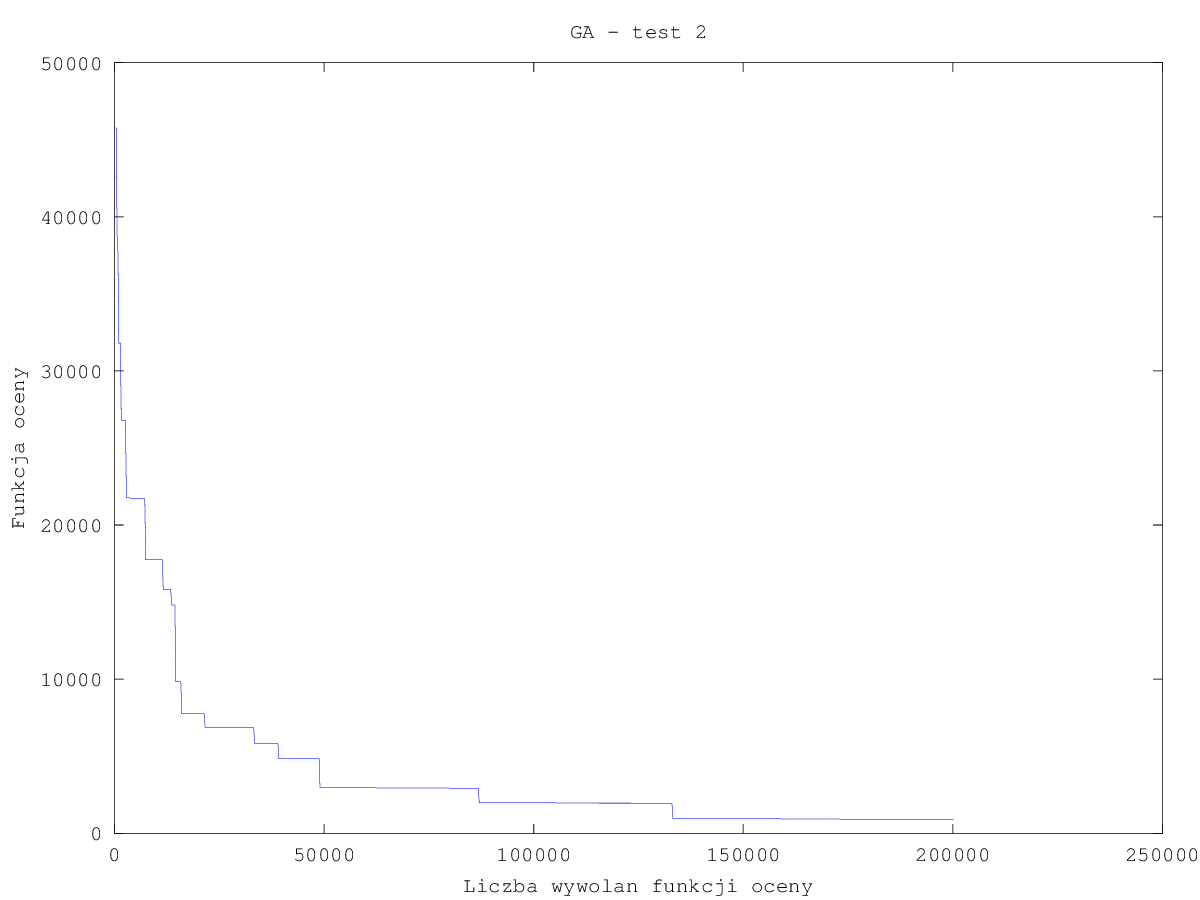
\includegraphics[width=10cm]{ga_test_2.png}
\end{figure}
\begin{figure}[H]
  \caption{Algorytm Roju Cząsteczek}
  \centering
    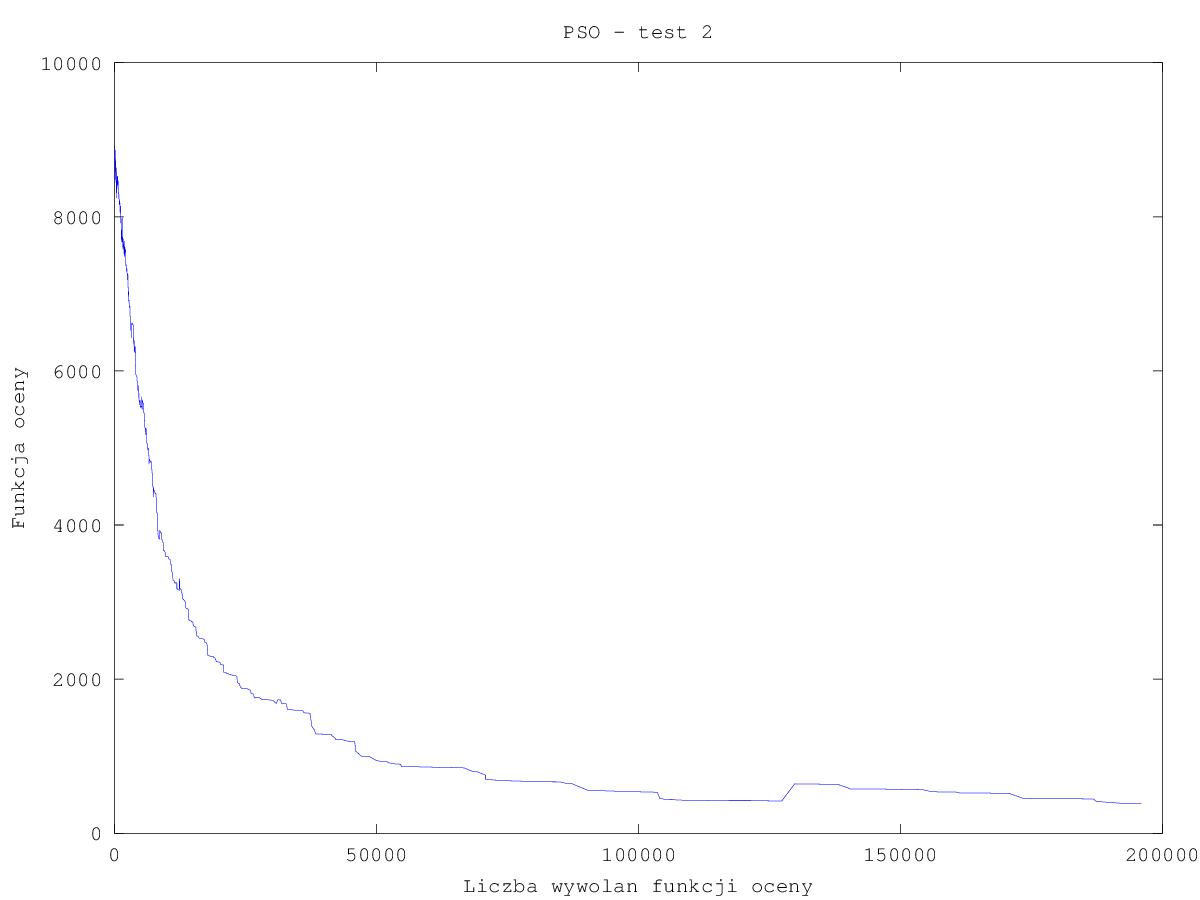
\includegraphics[width=10cm]{pso_2.png}
\end{figure}
\begin{figure}[H]
  \caption{Algorytm Adaptacyjny Tabu}
  \centering
    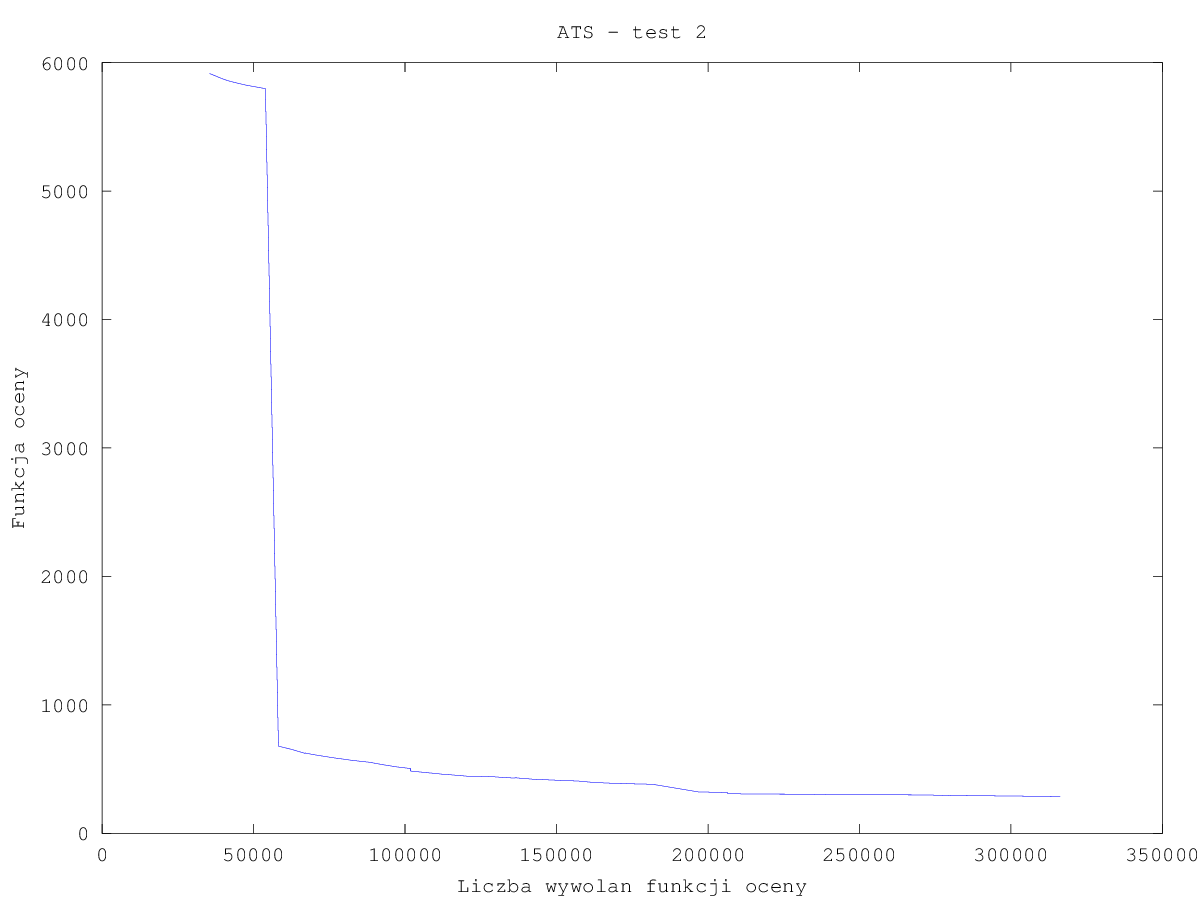
\includegraphics[width=10cm]{ats_test_2.png}
\end{figure}
Przedstwione wykresy potwierdzają wcześniej postawioną tezę o bardzo dużej liczbie odwołań do funkcji oceny dla algotytmu ATS. Początkowe rozwiązanie dla tego algotymu miało najniższą wartość funkcji oceny. Mimo początkowej wysokiej funkcji oceny dla algorytmu GA i PSO, końcowe rezultaty (wartości funkcji oceny) zostały w znaczący sposób pomniejszone, niestety dla PSO nie usuwając wszystkich ograniczeń twardych.
\subsection{Test 3}
\begin{table}[H]
\begin{center}

\begin{tabular}{ |c|c|c|c| }
\multicolumn{1}{r}{}
 &  \multicolumn{1}{c}{$$}
 & \multicolumn{1}{c}{$$} 
 \\
\cline{1-2}
$Liczba\ kursów$ & $72$\\
\cline{1-2}
$Liczba\ programów\ nauczania$ & $68$\\
\cline{1-2}
$Liczba\ dni$ & $5$ \\
\cline{1-2}
$Licza\ przedziałów\ czasowych$ & $5$ \\
\cline{1-2}
$Liczba\ ograniczeń$ & $382$ \\
\cline{1-2}
$Liczba\ sal$ & $16$ \\
\cline{1-2}
\end{tabular}
\end{center}
\caption {Specyfikacja danych - Test 3}
\end{table}
\par Wyniki działania algorytmów- ocena wygenerowanych planów zajęć: \\
Parametry dla algorytmów:
\begin{enumerate}
\item GA - liczba osobników: 200, liczba iteracji: 1000, szacowany czas działania algorytmu: 33 min
\item PSO - liczba cząsteczek: 20, liczba iteracji 5000, szacowany czas działania algorytmu: 90 min
\item ATS - czas działania: 16min
\end{enumerate}
\begin{table}[H]
\begin{center}

\begin{tabular}{ |l|l|l|l| }
\hline
 & $GA$ & $PSO$ & $ATS$\\
\hline
${H}_{1}\ Wykłady$ & $0$ & $0$ & $0$\\
\hline
$H_{2}\ Zajętość\ sali$ & $0$ & $0$ & $0$\\
\hline
$H_{3}\ Konflikty\ pomiędzy\ kursami$ & $0$ & $0$ & $0$ \\
\hline
$H_{4}\ Dostępność\ wykładowcy$ & $0$ & $1$ & $0$ \\
\hline
$S_{1}\ Wielkość\ sali$ & $82$ & $109$ & $12$ \\
\hline
$S_{2}\ Stabilność\ pomieszczenia$ & $50$ & $57$ & $125$ \\
\hline
$S_{3}\ Minimalna\ liczba\ dni$ & $20$ & $70$ & $40$ \\
\hline
$S_{4}\ Zwartość\ zajęć$ & $412$ & $202$ & $102$ \\
\hline
$Funkcja\ oceny$ & $564$ & $438$ & $279$ \\
\hline
\end{tabular}
\end{center}
\caption {Wyniki uzyskane przez poszczególne algorytmy}
\end{table}
Wyniki te potwierdzają najlepszą skuteczność działania algorytmu ATS, który generuje wykonywalny plan oraz jego funkcja oceny jest najniższa spośród pozostałych algorytmów. Warto również zauważyć dość dobrą skuteczność działania algorytmu GA, który eliminuje wszystkie ograniczenia twarde.
\par  Wykresy zmiany funkcji oceny w zależności od liczby odwołań do funkcji oceny dla poszczególnych algorytmów.
\begin{figure}[H]
  \caption{Algorytm Genetyczny}
  \centering
    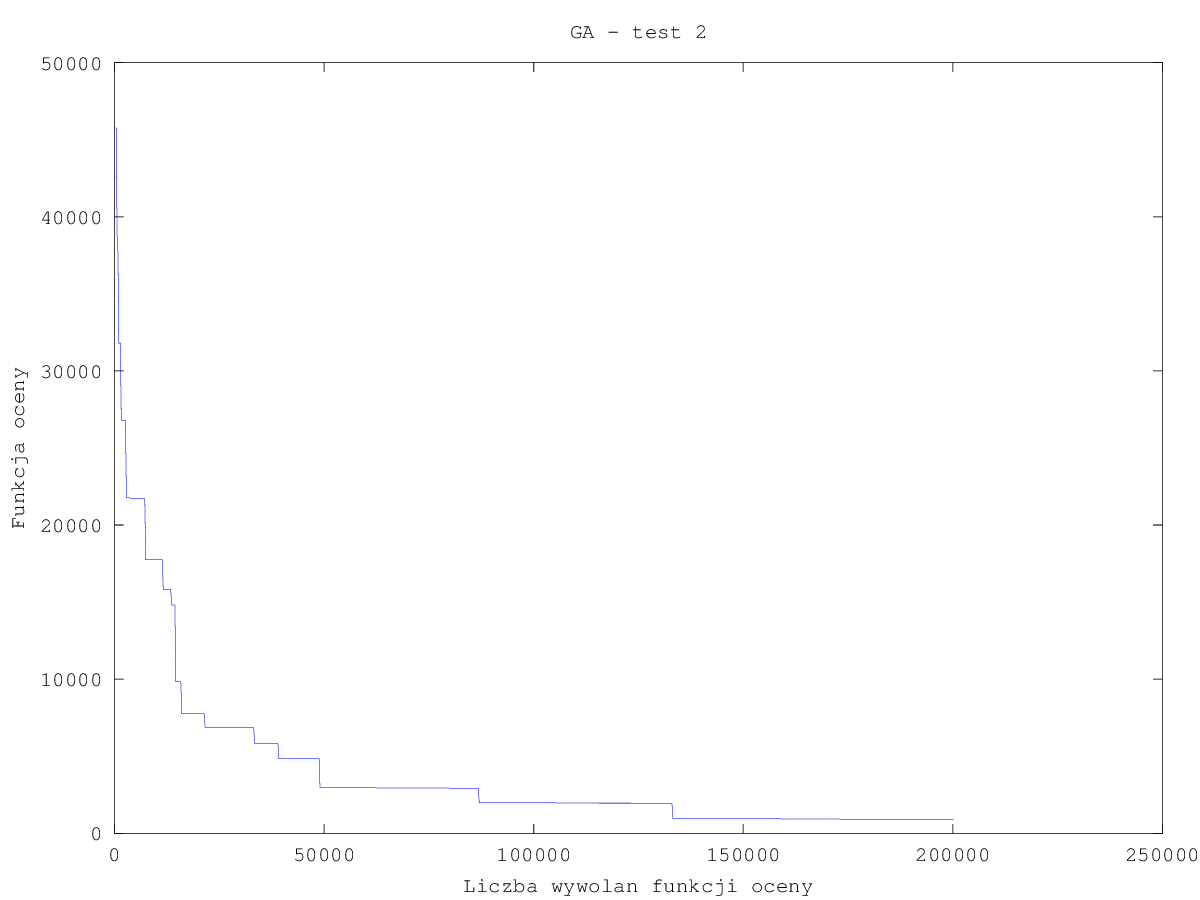
\includegraphics[width=10cm]{ga_test_2.png}
\end{figure}
\begin{figure}[H]
  \caption{Algorytm Roju Cząsteczek}
  \centering
    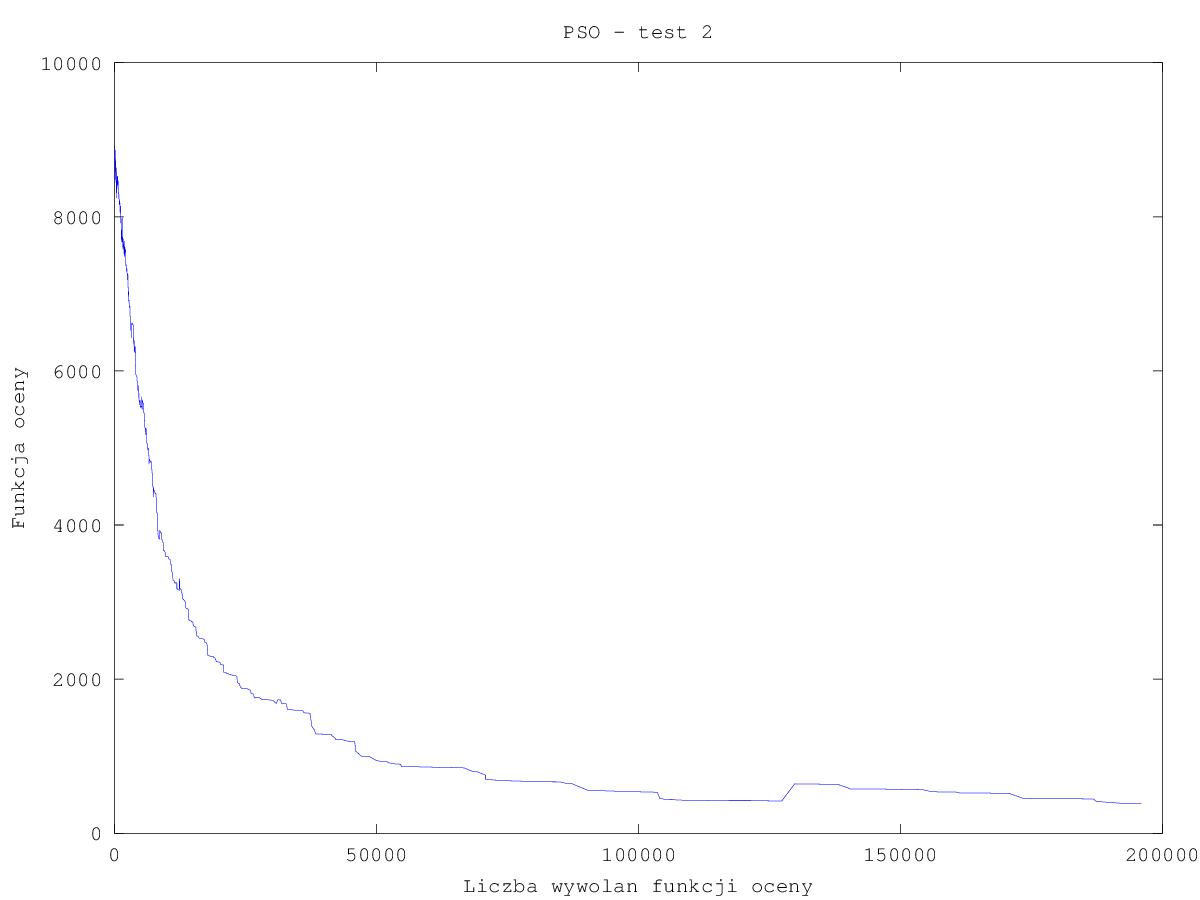
\includegraphics[width=10cm]{pso_2.png}
\end{figure}
\begin{figure}[H]
  \caption{Algorytm Adaptacyjny Tabu}
  \centering
    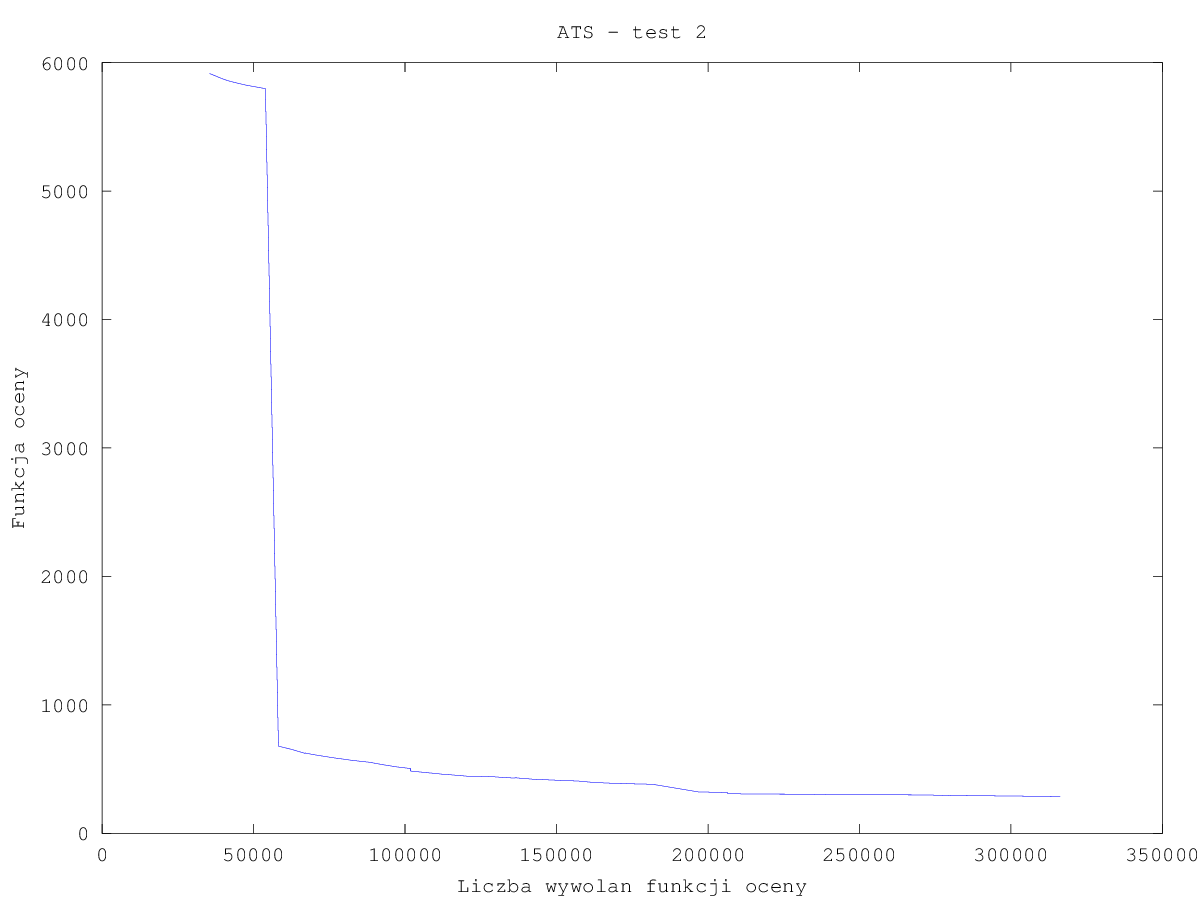
\includegraphics[width=10cm]{ats_test_2.png}
\end{figure}
\subsection{Dane szkolne}
Do działania na danych szkolnych zostały przystosowane dwa algorytmy: Algorytm Genetyczny i Algorytm Adaptacyjny Tabu.

\subsection{Podsumowanie działania algorytmów}
\par Algorytm Roju Cząsteczek nie dla wszystkich instancji był w stanie wygeneregować wykonywalny plan zajęć, pomimo stosunkowo długiego czasu działania. Algorytm ten nie daje gwarancji, że ograniczenia twarde zostaną całkowicie wyeliminowane.Ponadto metoda ta jest mało odporna na lokalne minima. Rozpatrywanie różnych modyfikacji algorytmu dało możliwość badawczego zapoznania się z tym jakże trudnym problemem, jakim jest układanie planu zajęć.
\par Algorytm Genetyczny jest również stosunkowo niepewnym rozwiązaniem, niedającym gwarancji o nie naruszeniu ograniczeń twardych. Głównym czynnikiem wpływającym na działanie algorytmu jest element losowy wprowadzony do niego, który w różny sposób tworzy początkowe rozwiązania. Zastosowanie zwiększonego współczynnika mutacji umożliwia wyjście algorytmu z lokalnego minimum. Algorytm mimo swojej prostoty, dla wybranych instancji uzyskał stosunkowo dobre wyniki.
\par Algorytm Adaptacyjny Tabu uzyskał dla większości instancji najlepsze wyniki. Algorytm ten gwarantuje zawsze spełnienie części z ograniczeń twardych $H_{2}-H_{4}$, nie zawsze zaś ograniczenia $H_{1}$. Ograniczenie ${H_{1}}$ jest naruszane w przypadku kiedy niemożliwe jest znalezienie przedziału czasu, gdzie może zostać przyporządkowany kurs nie naruszając $H_{2}-H_{4}$. ATS charakteryzuje się największą liczbą odwołań do funkcji oceny, w celu znalezienia optymalnego rozwiązania.







